%\setchapterpreamble[u]{\margintoc}
\chapter{Introduction}
\labch{intro}

% difference to 'drawing' -> different media
% shortcoming of computers to visualize this -> will draw enormous resources
% paintings are most often displayed though images -> no texture

\todo{this need at least some pictures in it}

The American Cambridge dictionary defines the word "picture" as
    
\dictcite{CAD}{picture}
\todo{add phonetic signs}
 
which right away separates between different media that can make up a picture.
If one were to look up the definitions of "drawing", "painting", and "photograph" as well, it becomes clear what distinguishes these three words:
\begin{itemize}
\item Paintings are only pictures that are made with paint.
\item A drawing is confined to pictures drawn with a pencil or pen.
\item Finally, a photograph is a picture taken with a camera.
\end{itemize}

All of these three methods could be used to picture the same image.
Yet, they will always give different results, as each medium comes with its limitations.\\
The painting will almost always deviate in its details from the original image, as paint tends to mix and flow.\\
The drawing will focus on edges and contours such that large colored regions have a somewhat smooth texture.\\
The photograph will limit an artist in showing anything more than the actual visual input.\\

Still, all of these techniques also have their characteristics that other techniques do not possess. \\
When comparing paintings to photographs, this becomes especially clear.
The layered texture of paintings varies vastly in thickness within a single painting.
A photograph can currently not capture and display this, as photographs are just projections of a 3D world onto a 2D plane.\\
This can not only be confirmed by art historians or the like but can be seen when looking at the industry of oil painting replicas.
Artists meticulously imitate every brushstroke of masterpieces such as The Starry Night by van Gogh or, most famously, the Mona Lisa by DaVinci.
There can only be a market for such replicas if actual painting and photos of paintings show enough of a difference.\\
Drawings suffer a different fate as they feature a rather two-dimensional structure and thus can be more easily copied and printed.
Subsequently, there are drawing applications on computers and tablets that have been useful tools for digital artists for over two decades now.
Due to technological advancement, it has become a feasible challenge to mimic the feel of pen on paper with styluses on glass tablets.\\
All of this makes it clear that the art of drawing has been subject to the digital revolution as much as the art of taking photographs.
\begin{marginfigure}
    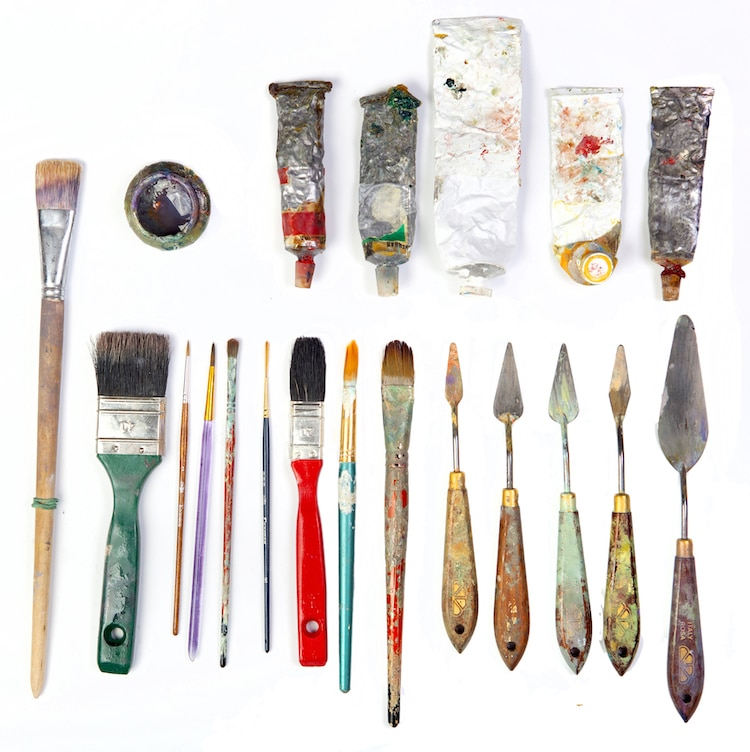
\includegraphics{oil_painting_tools}
    \caption[]{A typical set of brushes and spatulas used for oil paintings.} %Source:Kuznetcov_Konstantin/Shutterstock}
    \labfig{painting_tools}
\end{marginfigure}

But what about paintings?\\
Are there not also applications that try to imitate painting techniques, or 3D printed replicas of famous paintings?
Yes, there are, but it is clear that this comes with a lot more effort and limitations, as 3D scans and prints and real-time fluid simulations, are still far from perfect.\\
Even then, most digital content is consumed through 2D screens, which are not capable of displaying such content.
\begin{marginfigure}
    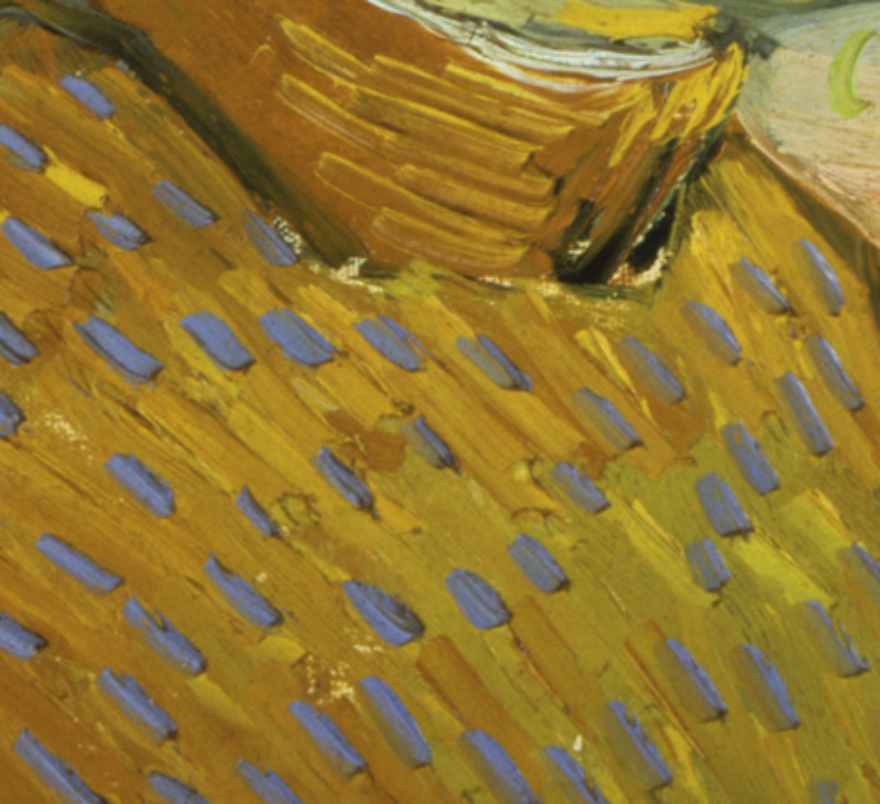
\includegraphics{images/cutout_orig}%
    \caption{Detailed brushstrokes in van Goghs painting 'The Little Arlesienne'.}
    \labfig{cutout_orig}%
\end{marginfigure}

So why even bother then, if all of these limitations are in place?\\
The development of technology in recent years suggests that the sky is the limit of what will be possible in future decades.
Coming up with ways of digitalizing paintings now will benefit development in the future.

Thus, the question arises how paintings could be digitalized.\\
One way to achieve this is 3D scans~\cite{3Dscan_art, 3Dscan_thesis} or gigapixel photographs of paintings~\cite{googleartproject}.
Both of these methods require much technological effort and money for each painting to be digitalized.\\
Another way imaginable would be to hire artists that already replicate paintings to do so in software.
Such an approach would also be combined with huge costs and take lots of time if it were to be realized for many paintings.

An interesting idea would be to combine the approach of re-drawing paintings with the latest technology in artificial intelligence and machine learning.
Such an approach would ideally not cost much (but the time and effort to develop the algorithm once).
At the same time, it would be able to approximate many images of paintings relatively fast automatically.

If it were possible to imitate many paintings this way easily, there would be benefits for other fields as well.
Conservation and restoration of paintings could be assisted digitally.
Art historians could quantify their research on the brushwork of artists.
More applications are imaginable, which means there is definitely a focus group for such technology.

So the question becomes: How could an image efficiently be described as a set of brushstrokes?

This thesis will propose a method to extract individual brushstrokes from a photograph of a painting.
All individual brushstrokes together should resemble the painting as well as possible.

As there is a vast realm of different painting techniques and materials, this work shall only deal with oil paintings and their brushstrokes.
Oil paintings and their brushstrokes have very characteristic visual features.
This will make it easier to evaluate them visually.
Even though many artists created oil paintings, van Gogh is probably the best-known artist associated with this field.
His works are well known, and thus there are many high-quality photographs of his paintings.
Also, most of the paintings by van Gogh show very clear brush strokes due to his style.

This thesis shall present a two-step approach to this problem.\\
First, a differentiable renderer is trained from a neural network.
The differentiable renderer generates images of single brushstrokes from parameters in a differentiable way.\\
This renderer should then be used to train a feed-forward prediction network.
A prediction network generates a set of parameters for a given input image which is meant to recreate the input.\\
If a feed-forward approach does not work, a backpropagation-based optimization procedure will be tested.
Such a procedure optimizes a set of brushstroke parameters directly such that they recreate the image together.\\
The resulting rendered paintings will be evaluated against other methods that claim to reconstruct images from brushstrokes.


As this thesis is part of a Master's degree in physics, the theoretical foundation in the next chapter is heavily motivated by neurobiological analogies.
Ideally, this should close the gap between computer vision and physics a little.\\
After building the theoretical foundations, an overview of common neural network architectures is presented.
The focus will be set on architectures which are relevant to the approach or the subsequent 'Related Works' chapter.\\
In 'Related Works' most of the relevant publications which combine paintings and computer vision will be introduced.
This chapter will be on the longer side, as 'artistic computer vision' (as it will be called in this thesis) is sort of a niche topic in computer vision.
Thus, a rather comprehensive overview is given such that the following approach can be better placed in this field.\\
Then the approach will be presented in two parts as it has done in this introduction. \\
Afterward, ablation experiments will be presented to show weaknesses and the influence of some decisions concerning the set-up.\\
The thesis will be wrapped up by a discussion of the results and how they compare to other works, followed by an outlook.

\paragraph{Allocation of individual contributions}
Arthur Heimbrecht worked on multiple projects during his Master's Thesis under the supervision of Johannes Haux, Dmytro Kotovenko, Matthias Wright, and Professor Björn Ommer.
The results, which are presented in this thesis, are the direct result of the continuing research by Dmytro Kotovenko, Matthias Wright, and Arthur Heimbrecht.
More precisely, the data set has been obtained by Matthias Wright and Arthur Heimbrecht.
Implementation, Training, and Experiments on the neural renderer have been performed by Dmytro Kotovenko, Matthias Wright, and Arthur Heimbrecht.
Dmytro Kotovenko has implemented the feed-forward approach.
The optimization procedure has been implemented by Arthur Heimbrecht and tested by Matthias Wright and Arthur Heimbrecht.
Professor Ommer suggested the project originally as part of an ongoing stream of research relating to study of art by means of computer vision
He also provided helpful guidance and critical feedback throughout this work.



As the presented approach relies on existing ideas but combined in a novel way, some focus in this thesis will lie on the implementation of the approach.
